\documentclass[crop,tikz]{standalone}
\usepackage{tkz-euclide}
\usetikzlibrary{arrows.meta}
\usetkzobj{all}
\usetikzlibrary{shapes}


\tikzstyle{myarrows}=[line width=1mm,draw=blue,-triangle 45,postaction={draw, line width=3mm, shorten >=4mm, -}]
\begin{document}

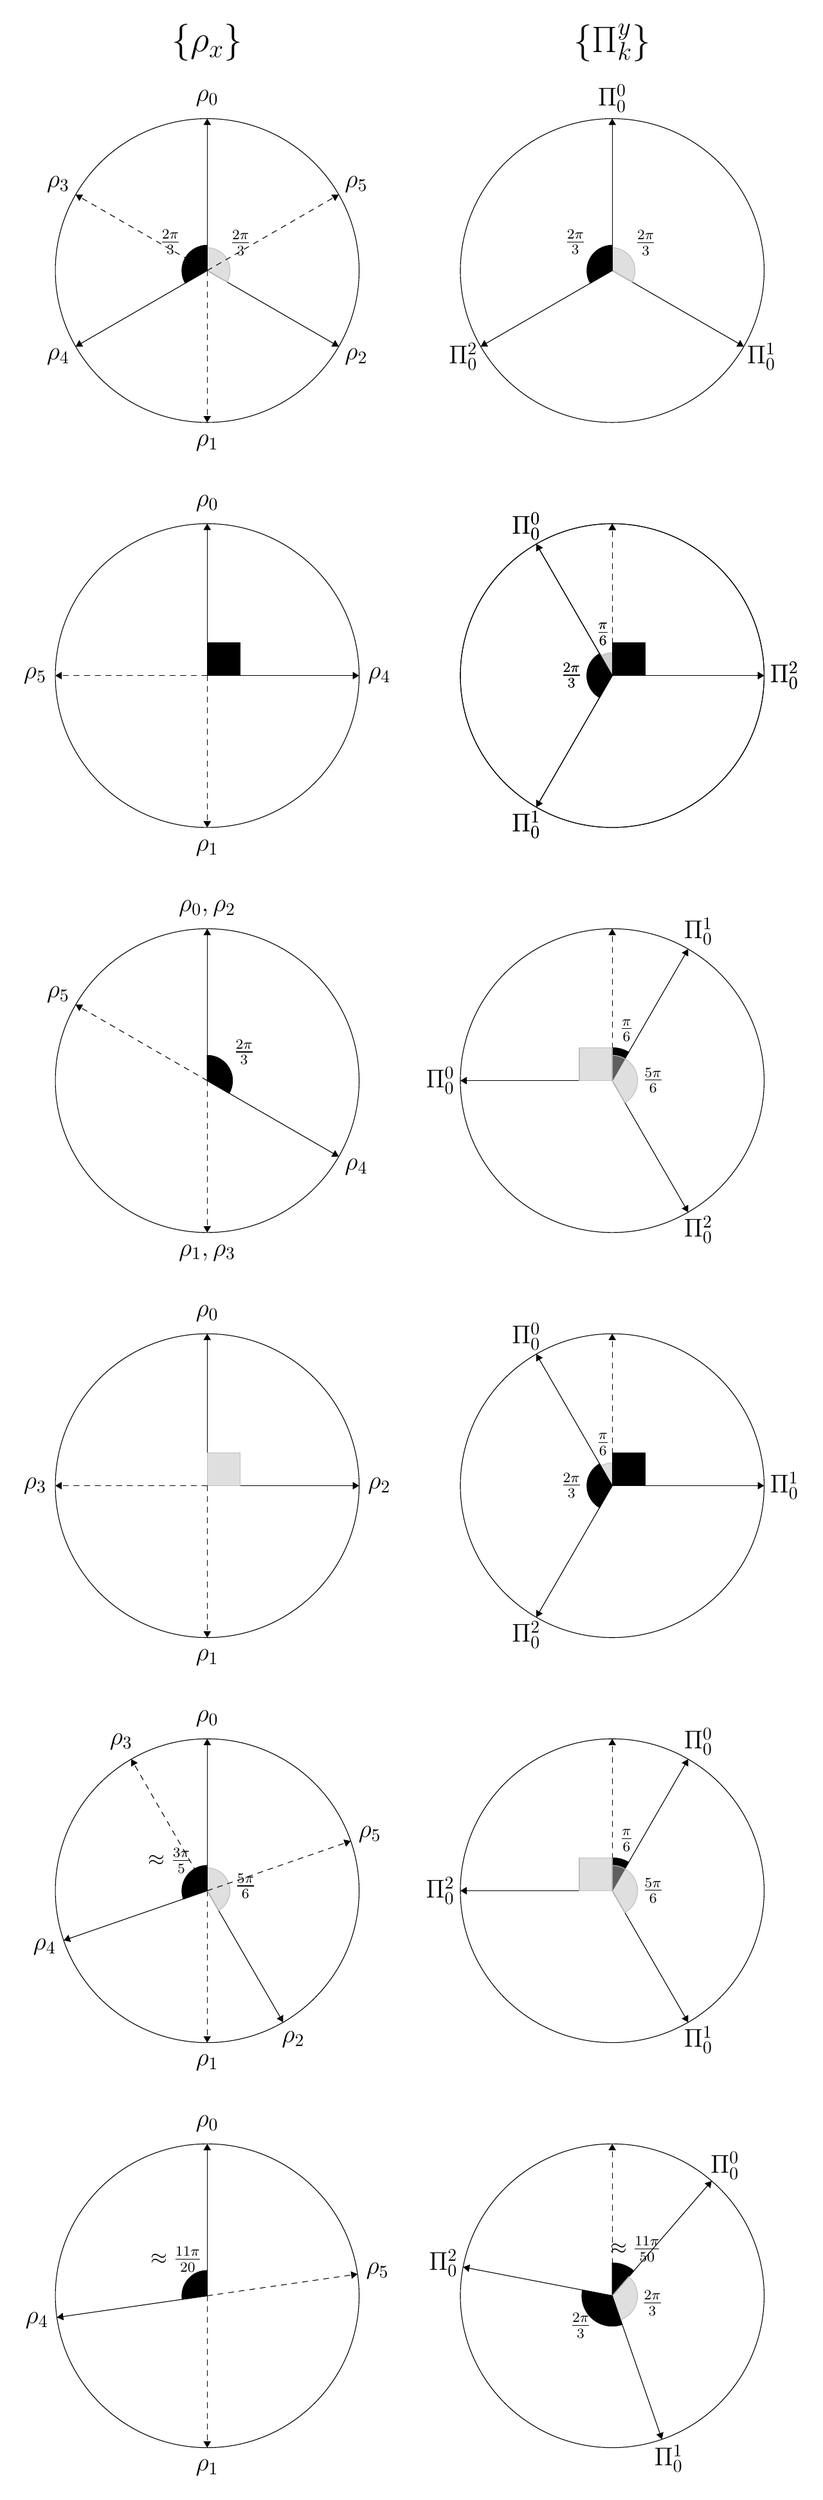
\begin{tikzpicture}[line cap=round, line join=round, >=Triangle]

\begin{scope}[ shift={(0,0)}]
\draw  (0,0) ellipse (3 and 3);


\draw[->]  (0,0) -- (0,3);
\draw (0,3.4) node {\Large $\rho_0$};



\begin{scope}[rotate=-180]
    \draw[->,dashed]  (0,0) -- (0,3);
	\draw (0,3.4) node {\Large $\rho_1$};
\end{scope}

\begin{scope}[rotate=-120]    
	\draw[->]  (0,0)  -- (0,3);
	\draw (0,3.4) node {\Large $\rho_2$};
	\draw [lightgray, fill, fill opacity=0.5]  (0,0) -- (90:0.45) arc (90:210:0.45) -- cycle;
	\node at (-0.8,0.3) {\large $\frac{2\pi}{3}$};
\end{scope}

\begin{scope}[rotate=60]    
	\draw[->,dashed]  (0,0)  -- (0,3);
	\draw (0,3.4) node {\Large $\rho_3$};
\end{scope}


\begin{scope}[rotate=120]    
	\draw[->]  (0,0)  -- (0,3);
	\draw (0,3.4) node {\Large $\rho_4$};
	\draw [shift={(0,0)}, fill] (0,0) -- (90:0.5) arc (90:-30:0.5) -- cycle;
\node at (0.85,0.35) {\large $\frac{2\pi}{3}$};
\end{scope}

\begin{scope}[rotate=-60]    
	\draw[->,dashed]  (0,0)  -- (0,3);
	\draw (0,3.4) node {\Large $\rho_5$};
\end{scope}

\node at (0,4.5) {\huge $\{\rho_x\}$ };
\end{scope}

%---------------------------------------------------------------------------------------------------
\begin{scope}[ shift={(8,0)}]
\draw  (0,0) ellipse (3 and 3);


\draw[->]  (0,0) -- (0,3);
\draw (0,3.4) node {\Large $\Pi^0_0$};




\begin{scope}[rotate=-120]    
	\draw[->]  (0,0)  -- (0,3);
	\draw (0,3.4) node {\Large $\Pi^1_0$};
	\draw [lightgray, fill, fill opacity=0.5]  (0,0) -- (90:0.45) arc (90:210:0.45) -- cycle;
	\node at (-0.8,0.3) {\large $\frac{2\pi}{3}$};
\end{scope}




\begin{scope}[rotate=120]    
	\draw[->]  (0,0)  -- (0,3);
	\draw (0,3.4) node {\Large $\Pi^2_0$};
	\draw [shift={(0,0)}, fill] (0,0) -- (90:0.5) arc (90:-30:0.5) -- cycle;
\node at (0.85,0.35) {\large $\frac{2\pi}{3}$};
\end{scope}



\node at (0,4.5) {\huge $\{\Pi^y_k\}$ };
\end{scope}

%---------------------------------------------------------------------------------------------------













\begin{scope}[ shift={(0,-8)}]
\draw  (0,0) ellipse (3 and 3);


\draw[->]  (0,0) -- (0,3);
\draw (0,3.4) node {\Large $\rho_0$};



\begin{scope}[rotate=-180]
    \draw[->,dashed]  (0,0) -- (0,3);
	\draw (0,3.4) node {\Large $\rho_1$};
\end{scope}

\begin{scope}[rotate=-90]    
	\draw[->]  (0,0)  -- (0,3);
	\draw (0,3.4) node {\Large $\rho_4$};
\draw [shift={(0,0)}, fill] (0,0) rectangle (-0.65,0.65);
\end{scope}

\begin{scope}[rotate=90]    
	\draw[->,dashed]  (0,0)  -- (0,3);
	\draw (0,3.4) node {\Large $\rho_5$};
\end{scope}
\end{scope}

\begin{scope}[ shift={(8,-8)}]
\draw  (0,0) ellipse (3 and 3);


\draw[->,dashed]  (0,0) -- (0,3);


\begin{scope}[rotate=30]    
	\draw[->]  (0,0)  -- (0,3);
	\draw (0,3.4) node {\Large $\Pi^0_0$};
	\draw [lightgray, fill, fill opacity=0.5]  (0,0) -- (90:0.45) arc (90:60:0.45) -- cycle;
	\node at (0.25,0.8) {\large $\frac{\pi}{6}$};
\end{scope}




\begin{scope}[rotate=150]    
	\draw[->]  (0,0)  -- (0,3);
	\draw (0,3.4) node {\Large $\Pi^1_0$};
	\draw [shift={(0,0)}, fill] (0,0) -- (90:0.5) arc (90:-30:0.5) -- cycle;
     \node at (0.7,0.4) {\large $\frac{2\pi}{3}$};
\end{scope}


\begin{scope}[rotate=-90]    
	\draw[->]  (0,0)  -- (0,3);
	\draw (0,3.4) node {\Large $\Pi^2_0$};
	\draw [shift={(0,0)}, fill] (0,0) rectangle (-0.65,0.65);
\end{scope}

\end{scope}











\begin{scope}[ shift={(0,-16)}]
\draw  (0,0) ellipse (3 and 3);


\draw[->]  (0,0) -- (0,3);
\draw (0,3.4) node {\Large $\rho_0,\rho_2$};



\begin{scope}[rotate=-180]
    \draw[->,dashed]  (0,0) -- (0,3);
	\draw (0,3.4) node {\Large $\rho_1,\rho_3$};
\end{scope}




\begin{scope}[rotate=-120]    
	\draw[->]  (0,0)  -- (0,3);
	\draw (0,3.4) node {\Large $\rho_4$};
	\draw [shift={(0,0)}, fill] (0,0) -- (90:0.5) arc (90:210:0.5) -- cycle;
\node at (-	0.85,0.35) {\large $\frac{2\pi}{3}$};
\end{scope}

\begin{scope}[rotate=60]    
	\draw[->,dashed]  (0,0)  -- (0,3);
	\draw (0,3.4) node {\Large $\rho_5$};
\end{scope}


\end{scope}

%---------------------------------------------------------------------------------------------------
\begin{scope}[ shift={(8,-16)}]
\draw  (0,0) ellipse (3 and 3);


\draw[->,dashed]  (0,0) -- (0,3);


\begin{scope}[rotate=-30]    
	\draw[->]  (0,0)  -- (0,3);
	\draw (0,3.4) node {\Large $\Pi^1_0$};
	\draw [fill]  (0,0) -- (90:0.65) arc (90:120:0.65) -- cycle;
	\node at (-0.25,1) {\large $\frac{\pi}{6}$};
\end{scope}




\begin{scope}[rotate=-150]    
	\draw[->]  (0,0)  -- (0,3);
	\draw (0,3.4) node {\Large $\Pi^2_0$};
	\draw [lightgray, fill, fill opacity=0.5] (0,0) -- (90:0.5) arc (90:240:0.5) -- cycle;
     \node at (-0.7,0.4) {\large $\frac{5\pi}{6}$};
\end{scope}


\begin{scope}[rotate=90]    
	\draw[->]  (0,0)  -- (0,3);
	\draw (0,3.4) node {\Large $\Pi^0_0$};
	\draw [shift={(0,0)},lightgray, fill, fill opacity=0.5] (0,0) rectangle (0.65,0.65);
\end{scope}

\end{scope}

%---------------------------------------------------------------------------------------------------









\begin{scope}[ shift={(0,-24)}]
\draw  (0,0) ellipse (3 and 3);


\draw[->]  (0,0) -- (0,3);
\draw (0,3.4) node {\Large $\rho_0$};



\begin{scope}[rotate=-180]
    \draw[->,dashed]  (0,0) -- (0,3);
	\draw (0,3.4) node {\Large $\rho_1$};
\end{scope}

\begin{scope}[rotate=-90]    
	\draw[->]  (0,0)  -- (0,3);
	\draw (0,3.4) node {\Large $\rho_2$};
	\draw [shift={(0,0)},lightgray, fill, fill opacity=0.5] (0,0) rectangle (-0.65,0.65);
\end{scope}

\begin{scope}[rotate=90]    
	\draw[->,dashed]  (0,0)  -- (0,3);
	\draw (0,3.4) node {\Large $\rho_3$};
\end{scope}

%---------------------------------------------------------------------------------------------------

\end{scope}
\begin{scope}[ shift={(8,-8)}]
\draw  (0,0) ellipse (3 and 3);


\draw[->,dashed]  (0,0) -- (0,3);


\begin{scope}[rotate=30]    
	\draw[->]  (0,0)  -- (0,3);
	\draw (0,3.4) node {\Large $\Pi^0_0$};
	\draw [lightgray, fill, fill opacity=0.5]  (0,0) -- (90:0.45) arc (90:60:0.45) -- cycle;
	\node at (0.25,0.8) {\large $\frac{\pi}{6}$};
\end{scope}




\begin{scope}[rotate=150]    
	\draw[->]  (0,0)  -- (0,3);
	\draw (0,3.4) node {\Large $\Pi^1_0$};
	\draw [shift={(0,0)}, fill] (0,0) -- (90:0.5) arc (90:-30:0.5) -- cycle;
     \node at (0.7,0.4) {\large $\frac{2\pi}{3}$};
\end{scope}


\begin{scope}[rotate=-90]    
	\draw[->]  (0,0)  -- (0,3);
	\draw (0,3.4) node {\Large $\Pi^2_0$};
	\draw [shift={(0,0)}, fill] (0,0) rectangle (-0.65,0.65);
\end{scope}

\end{scope}

\begin{scope}[ shift={(8,-24)}]
\draw  (0,0) ellipse (3 and 3);


\draw[->,dashed]  (0,0) -- (0,3);


\begin{scope}[rotate=30]    
	\draw[->]  (0,0)  -- (0,3);
	\draw (0,3.4) node {\Large $\Pi^0_0$};
	\draw [lightgray, fill, fill opacity=0.5]  (0,0) -- (90:0.45) arc (90:60:0.45) -- cycle;
	\node at (0.25,0.8) {\large $\frac{\pi}{6}$};
\end{scope}




\begin{scope}[rotate=150]    
	\draw[->]  (0,0)  -- (0,3);
	\draw (0,3.4) node {\Large $\Pi^2_0$};
	\draw [shift={(0,0)}, fill] (0,0) -- (90:0.5) arc (90:-30:0.5) -- cycle;
     \node at (0.7,0.4) {\large $\frac{2\pi}{3}$};
\end{scope}


\begin{scope}[rotate=-90]    
	\draw[->]  (0,0)  -- (0,3);
	\draw (0,3.4) node {\Large $\Pi^1_0$};
	\draw [shift={(0,0)}, fill] (0,0) rectangle (-0.65,0.65);
\end{scope}

\end{scope}










%---------------------------------------------------------------------------------------------------
\begin{scope}[ shift={(0,-32)}]
\draw  (0,0) ellipse (3 and 3);


\draw[->]  (0,0) -- (0,3);
\draw (0,3.4) node {\Large $\rho_0$};



\begin{scope}[rotate=-180]
    \draw[->,dashed]  (0,0) -- (0,3);
	\draw (0,3.4) node {\Large $\rho_1$};
\end{scope}

\begin{scope}[rotate=-150]    
	\draw[->]  (0,0)  -- (0,3);
	\draw (0,3.4) node {\Large $\rho_2$};
	\draw [lightgray, fill, fill opacity=0.5]  (0,0) -- (90:0.45) arc (90:240:0.45) -- cycle;
	\node at (-0.7,0.3) {\large $\frac{5\pi}{6}$};
\end{scope}

\begin{scope}[rotate=30]    
	\draw[->,dashed]  (0,0)  -- (0,3);
	\draw (0,3.4) node {\Large $\rho_3$};
\end{scope}


\begin{scope}[rotate=109.1]    
	\draw[->]  (0,0)  -- (0,3);
	\draw (0,3.4) node {\Large $\rho_4$};
	\draw [shift={(0,0)}, fill] (0,0) -- (90:0.5) arc (90:-30+10.9:0.5) -- cycle;
\node at (0.8,0.5) {\large $\approx\frac{3\pi}{5}$};
\end{scope}

\begin{scope}[rotate=-70.9]    
	\draw[->,dashed]  (0,0)  -- (0,3);
	\draw (0,3.4) node {\Large $\rho_5$};
\end{scope}

\end{scope}

%---------------------------------------------------------------------------------------------------
%---------------------------------------------------------------------------------------------------
\begin{scope}[ shift={(8,-32)}]
\draw  (0,0) ellipse (3 and 3);


\draw[->,dashed]  (0,0) -- (0,3);


\begin{scope}[rotate=-30]    
	\draw[->]  (0,0)  -- (0,3);
	\draw (0,3.4) node {\Large $\Pi^0_0$};
	\draw [fill]  (0,0) -- (90:0.65) arc (90:120:0.65) -- cycle;
	\node at (-0.25,1) {\large $\frac{\pi}{6}$};
\end{scope}




\begin{scope}[rotate=-150]    
	\draw[->]  (0,0)  -- (0,3);
	\draw (0,3.4) node {\Large $\Pi^1_0$};
	\draw [lightgray, fill, fill opacity=0.5] (0,0) -- (90:0.5) arc (90:240:0.5) -- cycle;
     \node at (-0.7,0.4) {\large $\frac{5\pi}{6}$};
\end{scope}


\begin{scope}[rotate=90]    
	\draw[->]  (0,0)  -- (0,3);
	\draw (0,3.4) node {\Large $\Pi^2_0$};
	\draw [shift={(0,0)},lightgray, fill, fill opacity=0.5] (0,0) rectangle (0.65,0.65);
\end{scope}

\end{scope}












%---------------------------------------------------------------------------------------------------
\begin{scope}[ shift={(0,-40)}]
\draw  (0,0) ellipse (3 and 3);


\draw[->]  (0,0) -- (0,3);
\draw (0,3.4) node {\Large $\rho_0$};



\begin{scope}[rotate=-180]
    \draw[->,dashed]  (0,0) -- (0,3);
	\draw (0,3.4) node {\Large $\rho_1$};
\end{scope}


\begin{scope}[rotate=98.2]    
	\draw[->]  (0,0)  -- (0,3);
	\draw (0,3.4) node {\Large $\rho_4$};
	\draw [shift={(0,0)}, fill] (0,0) -- (90:0.5) arc (90:-30+21.8:0.5) -- cycle;
\node at (0.8,0.5) {\large $\approx\frac{11\pi}{20}$};
\end{scope}

\begin{scope}[rotate=-81.8]    
	\draw[->,dashed]  (0,0)  -- (0,3);
	\draw (0,3.4) node {\Large $\rho_5$};
\end{scope}

\end{scope}

%---------------------------------------------------------------------------------------------------
%---------------------------------------------------------------------------------------------------
\begin{scope}[ shift={(8,-40)}]
\draw  (0,0) ellipse (3 and 3);


\draw[->,dashed]  (0,0) -- (0,3);


\begin{scope}[rotate=-40.89]    
	\draw[->]  (0,0)  -- (0,3);
	\draw (0,3.4) node {\Large $\Pi^0_0$};
	\draw [fill]  (0,0) -- (90:0.65) arc (90:90+40.89:0.65) -- cycle;
	\node at (-0.25,1) {\large $\approx \frac{11\pi}{50}$};
\end{scope}




\begin{scope}[rotate=-160.89]    
	\draw[->]  (0,0)  -- (0,3);
	\draw (0,3.4) node {\Large $\Pi^1_0$};
	\draw [lightgray, fill, fill opacity=0.5] (0,0) -- (90:0.5) arc (90:210:0.5) -- cycle;
     \node at (-0.7,0.4) {\large $\frac{2\pi}{3}$};
\end{scope}


\begin{scope}[rotate=79.10]    
	\draw[->]  (0,0)  -- (0,3);
	\draw (0,3.4) node {\Large $\Pi^2_0$};
		\draw [fill] (0,0) -- (90:0.6) arc (90:210:0.6) -- cycle;
		\node at (-0.7,0.5) {\large $\frac{2\pi}{3}$};

\end{scope}

\end{scope}

\end{tikzpicture}

\end{document}